\documentclass[useAMS,usenatbib]{mn2e}
\usepackage{footnote,graphicx,natbib,color,multirow,amsmath,url,amssymb,tabularx,hyperref,amssymb, mathtools, listings, float}
\usepackage{aas_macros}

\hypersetup{draft,
    colorlinks,
    citecolor=blue,
    filecolor=black,
    linkcolor=black,
    urlcolor=black
}

\def\lesssim{\mathrel{\hbox{\rlap{\hbox{\lower3pt\hbox{$\sim$}}}\hbox{\raise2pt\hbox{$<$}}}}}

\definecolor{check}{rgb}{1,0,0}
\def\check		{\color{check}}

\begin{document}

\title[\textsc{snitch}: inferring quenching histories]{SNITCH: Seeking a simple, comparative star formation history inference tool}
\author[Smethurst et al. 2018]{R. ~J. ~Smethurst,$^{1}$  et al.
\\ $^1$ School of Physics and Astronomy, The University of Nottingham, University Park, Nottingham, NG7 2RD, UK
% \\ $^2$ Oxford Astrophysics, Department of Physics, University of Oxford, Denys Wilkinson Building, Keble Road, Oxford, OX1 3RH, UK
}

\maketitle

\begin{abstract}
We present \textsc{snitch}, an open source code written in \emph{Python}, developed to infer a simple toy model of the star formation history of a galaxy spectrum from the emission and absorption features. \textsc{snitch} utilises FSPS, the MaNGA DAP and \emph{emcee} in order to infer the $[Z, t_q, \log \tau]$ parameters which best  describe an exponentially declining quenching history to fit the input spectral features. This code was written for use on the MaNGA spectral data cubes but is customisable by a user so that it can be used for any scenario where a galaxy spectrum has been obtained, or spectral feature measurements have been provided. This code is not intended for an accurate inference of a single spectrum SFH but as a comparison of SFHs across many different spectra, either for IFU data or across a large galaxy sample.
\end{abstract}

\begin{keywords}
software -- description
\end{keywords}

\section{Introduction}

Whilst there are many publicly available codes which provide a full spectral fit to a galaxy spectrum in order to determine its star formation history (SFH), there are few providing a simpler, quicker inference of a toy model of SFH for comparative studies. 

Here we present an open source \emph{Python} software which uses Bayesian statistics and MCMC methods to infer a simple toy model of SFH from the absorption and emission features of a galaxy (or IFU) spectrum. 

%QUIDDITCH: QUenching hIstory Determination with absorption inDices and emIssion lines using bayesian TeCHniques

%QUIDDITCH: QUenching Investigations with Data-Driven Inference TeCHniques

Herein we describe our SFH inference code, \textsc{snitch} (bayeSian iNference, given emIssion and absorpTion features, of quenChing Histories), in Section~\ref{sec:code}, the expected output of the code in Section~\ref{sec:output}, along with the rigorous testing procedures applied to \textsc{snitch} in Section~\ref{sec:test}. Where necessary we adopt the Planck 2015 \citep{planck16} cosmological parameters with $(\Omega_m, \Omega_{\lambda}, h) = (0.31, 0.69, 0.68)$. 

\section{Description of Code}\label{sec:code}

As a black box, \textsc{snitch} takes absorption and emission spectral features and their associated errors as inputs, assumes a simple SFH model and convolves it with a SPS to generate a synthetic spectra. These synthetic spectra are then fitted to give resulting predicted absorption and emission spectral features which the code uses to infer the best fit model using Bayesian statistics and MCMC methods. 

We describe this process below, first defining our toy model of SFH, describing how we convolve this with SPS models to produce synthetic spectra (Section~\ref{sec:fsps}), how these spectra are then fitted to provide predicted model spectral features (Section~\ref{sec:dap}) and then how these are used to infer the best fit SFH given the input parameters (Section~\ref{sec:emcee}). 

\subsection{Star Formation History Model}\label{sec:sfh}

The SFH used in this code was first described in \cite{smethurst15}. We have reproduced its description here. The quenched star formation history of a galaxy can be simply modelled as an exponentially declining star formation rate (SFR) across cosmic time as:
\begin{equation}\label{sfh}
SFR =
\begin{cases}
I_{sfr}(t_q) & \text{if } t \leq t_q \\
I_{sfr}(t_q) \times exp{\left( \frac{-(t-t_{q})}{\tau}\right)} & \text{if } t > t_q 
\end{cases}
\end{equation}
where $t_{q}$ is the onset time of quenching, $\tau$ is the timescale over which the quenching occurs and $I_{sfr}$ is an initial constant star formation rate dependent on $t_q$.  A smaller $\tau$ value corresponds to a rapid quench, whereas a larger $\tau$ value corresponds to a slower quench. This model is clearly not a fully hydrodynamical simulation, it is a deliberately simple model built in order to test our understanding of the evolution of galaxy, or stellar, populations. This SFH model has previously been shown to appropriately characterise quenching galaxies \citep{weiner06, martin07, noeske07,schawinski14}. For galaxies which are still star forming, this model results in a constant SFR.

\begin{figure*}
\centering
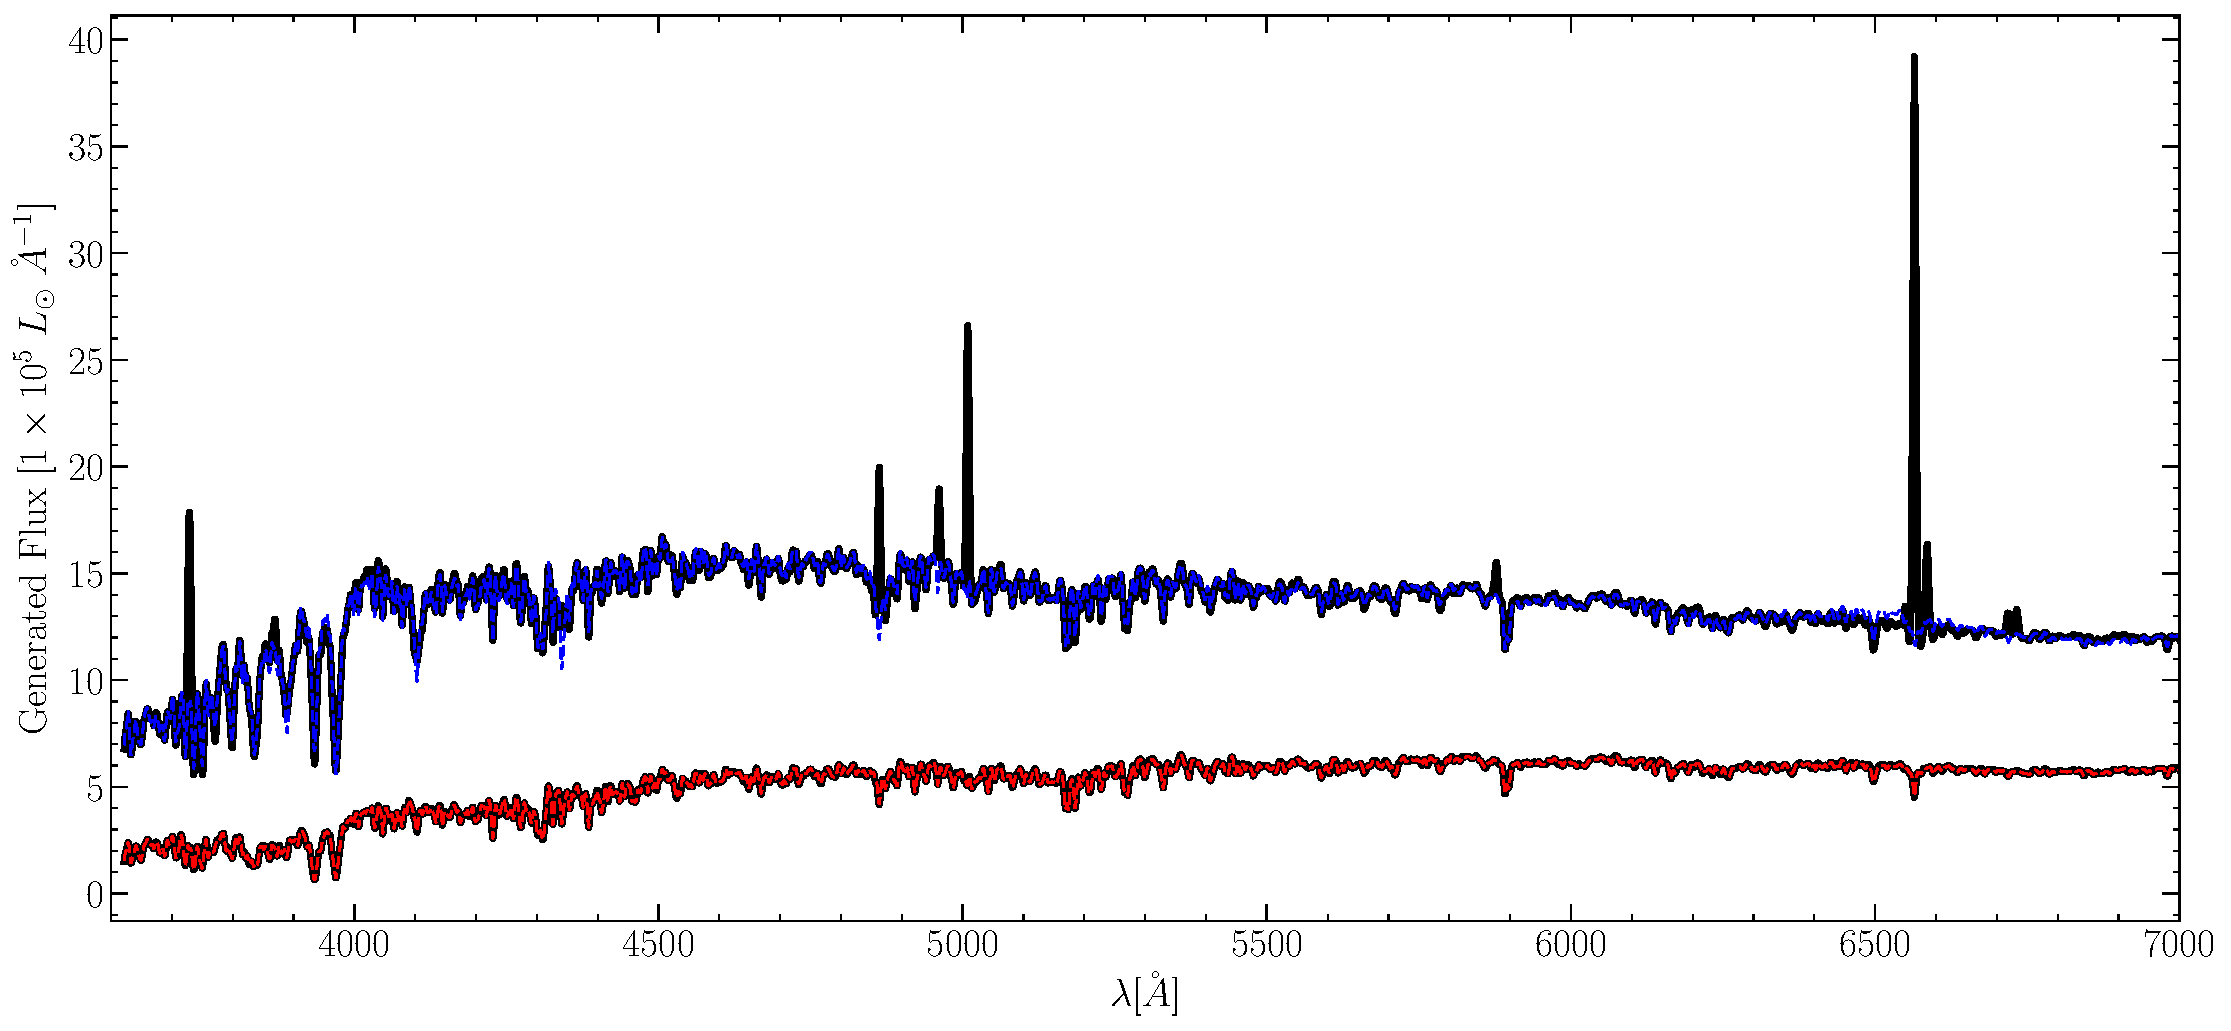
\includegraphics[width=\textwidth]{../figures/example_spectra_fits_tq_10_tau_1_Z_1_t_obs_10_red_14_blue_AA.png}
\caption{Example synthetic spectra constructed using FSPS, shown by the black solid lines, both with a SFH of $[Z,~t_q,~\tau]~=~[1~Z_{\odot},~10.0~\rm{Gyr},~0.5~\rm{Gyr}]$. We also show the fit to the continuum returned by the MaNGA DAP (see Section~\ref{sec:dap}) shown by the red dashed line for the spectra observed at $t_{\rm{obs}} = 13.8~\rm{Gyr}$ and the blue dashed line for the spectra observed at $t_{\rm{obs}} = 10.4~\rm{Gyr}$ soon after quenching has begun.}
\label{fig:spectrafit}
\end{figure*}

Here, we assume that all galaxies formed at a time $t=0~\rm{Gyr}$ with an initial burst of star formation, $I_{sfr}(t_q)$. This initial constant star formation rate must be defined in order to ensure the `model' galaxy  has a reasonable stellar mass by $z\sim0$. This value will be dependent on the epoch at which quenching is modelled to occur, hence the dependence of this initial star formation rate on quenching time in Equation~\ref{sfh}. 

\citet[][Equation 1]{peng10} define a relation between the average specific SFR ($\rm{sSFR}=SFR/M_*$) and redshift by fitting to measurements of the mean sSFR of blue star forming galaxies from SDSS, zCOSMOS and literature values from \cite{elbaz07} and \cite{daddi07} measured at increasing redshifts with data from the GOODS survey:
\begin{equation}\label{eq:peng}
sSFR(m,t) = 2.5 \left( \frac{m}{10^{10} M_{\odot}} \right)^{-0.1} \left(\frac{t}{3.5 ~\rm{Gyr}}\right)^{-2.2} \rm{Gyr}^{-1}.
\end{equation}
Beyond $z \sim 2$ the characteristic sSFR flattens and is roughly constant back to $z\sim6$. This flattening can be seen across similar observational data \citep{peng10, gonzalez10, bethermin12}; the cause is poorly understood but may reflect a physical limit to the sSFR of a galaxy. 

Motivated by these observations, the relation defined in \citet{peng10} is taken up to a cosmic time of $t=3~\rm{Gyr}$ ($z \sim 2.3$) and prior to this the value of the sSFR at $t=3~\rm{Gyr}$ is used. At the point of quenching, $t_{q}$, the SFH models are therefore defined to have an $I_{sfr}(t_q)$ which lies on this relationship for the sSFR, for a galaxy with mass, $m = 10^{10.27} M_{\odot}$. This choice of $I_{sfr}(t_q)$ is an important one to produce realistic synthetic galaxy properties, however does not impact on the predicted spectral features output by the model as it is merely a normalisation factor on the SFH. The SFH parameters $[t_q, \log \tau]$, which set the shape of the SFH, and the metallicity, $Z$, which can affect the strength of a spectral feature, are the crucial parameters.

\subsection{Synthetic spectra generation}\label{sec:fsps}

We then employ stellar population synthesis models (SPS) in order to construct synthetic spectra with the SFHs defined in Section~\ref{sec:sfh}. These synthetic spectra will be measured the same as an observed spectra (see Section~\ref{sec:dap}) in order to make a direct comparison using Bayesian statistics (see Section~\ref{sec:emcee}) to determine the `best fit' SFH model for a given spectral features input. 

In order to derive a realistic synthetic spectra with our defined SFHs we utilised the Flexible Stellar Population Synthesis (FSPS) Model\footnote{\url{https://github.com/cconroy20/fsps}} code of \cite{conroy09} and \citet{conroy10}, which is written in \texttt{FORTRAN}, in conjunction with an existing \emph{Python} wrapper\footnote{\url{http://dfm.io/python-fsps/current/}} by \cite{python_fsps}. SPS methods rely on stellar evolution calculations during all stages of stellar life, stellar spectral libraries, dust models and initial mass functions (IMFs) to translate the evolution of a hypothetical number of stars of varying ages and metallicities into a predicted integrated spectrum. FSPS also integrates \texttt{CLOUDY} \citep{ferland13} into its output so that stellar emission lines can be synthesised along with the stellar continuum. 

The FSPS Python wrapper makes it possible to generate spectra (or magnitudes) for any arbitrary stellar population in just two lines of \emph{Python} code. 
% For example:

% \begin{lstlisting}[language=Python]
% sp = fsps.StellarPopulation(
% 	zmet=18, sfh=3, 
% 	dust_type=2, imf_type=1,
% 	add_neb_emission=True,  
% 	add_dust_emission=True)
% sp.set_tabular_sfh(age = ages, sfr=sfrs)
% \end{lstlisting}

\begin{figure*}
\centering
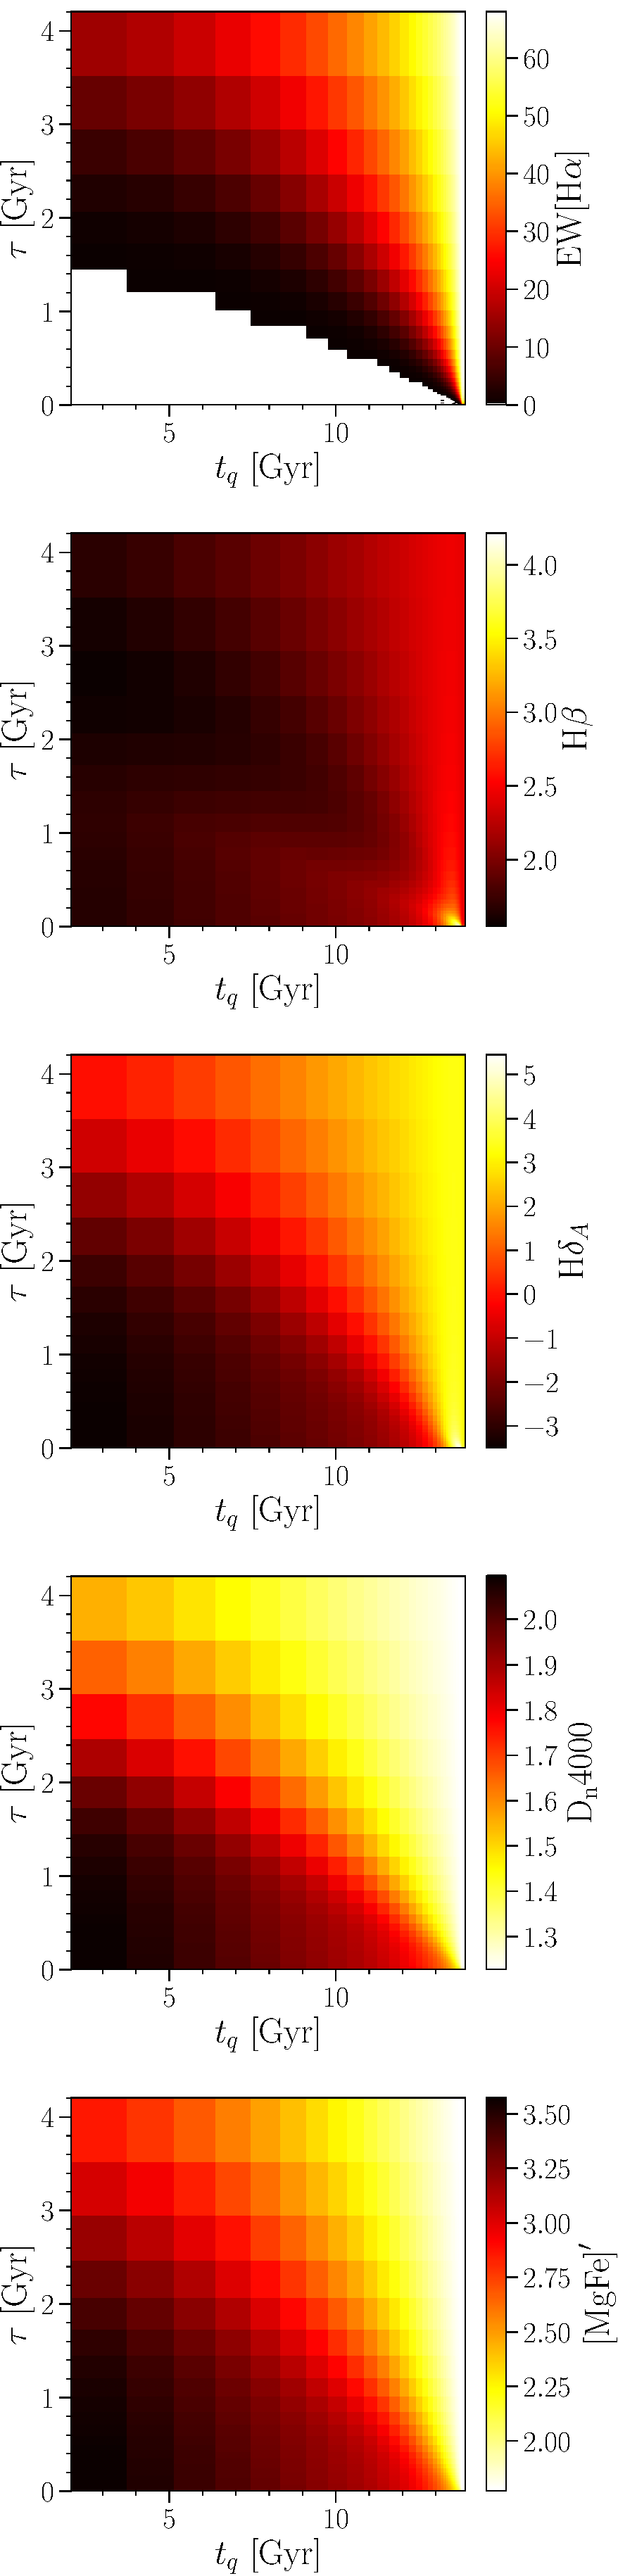
\includegraphics[width=\textwidth]{../figures/fsps_rainbow_spectral_features.pdf}
\caption{The variation of model spectral features across the logarithmically binned two dimensional $[t_q, \log \tau]$ parameter space measured at $t_{obs}=13.8~\rm{Gyr}$ and solar metallicity, $Z=Z_{\odot}$. The features shown from left to right are the equivalent width of the $H\alpha$ emission line and the spectral absorption indices $\rm{H}\beta$, MgFe', $\rm{H}\delta_A$ and $\rm{D}_n4000$,. Note that when a model is no longer star forming, the fitting code cannot measure an equivalent width of $H\alpha$ therefore these values are masked out in the bottom left corner of the left panel. This figure shows how each feature is sensitive to the changing SFH and how they can be used to break the degeneracies that plague photometric studies of SFH. }
\label{fig:rainbow}
\end{figure*}



In \textsc{snitch} we set up the FSPS models to produce spectra using the Padova isochrones \citep{girardi02} and MILES spectral library \citep{vazdekis16} with nebular emission, emission from dust \cite{draineli07}, a \cite{chabrier03} IMF and a \cite{calzetti00} dust extinction curve. We also smooth the generated synthetic spectra to have the minimum velocity dispersion measurable by MaNGA, $77~\rm{km}~{s}^{-1}$ \citep{bundy15}. Spectra are generated for the 22 metalicities provided in the MILES models, ranging from $0.011~Z_{\odot}$ to $1.579~Z_{\odot}$ across a logarithmic age range spanning the Universe's history. FSPS does not allow for chemical enrichment of stellar birth material with time, i.e. the metallicity is kept constant for a given SFH at all epochs.\footnote{Whilst we could attempt to provide a feature to implement chemical enrichment into these models this would firstly be full of uncertainty (the propagation of which would be unquantifiable) and secondly move us out of the regime of a toy SFH model and into hydrodynamic simulation territory. } These spectra are generated across a logarithmically spaced 4-dimensional array in $[t_{obs},~Z,~t_q,~\tau]$ in order to facilitate faster run time during inference (see Section~\ref{sec:emcee}).

Two example synthetic spectra generated with FSPS for solar metallicity are shown by the solid black line in Figure~\ref{fig:spectrafit}. Note that FSPS generates spectra with flux units $L_{\odot}~\rm{Hz}^{-1}$, but that our fitting procedure (see Section~\ref{sec:dap}) requires the flux in units of $\rm{\AA}^{-1}$. The fits are shown by the red dashed line for a spectra which has already quenched with $[Z,~t_q,~\tau] = [1~Z_{\odot},~11.5~\rm{Gyr},~0.1~\rm{Gyr}]$ and by the blue dashed line for a spectra which still has some residual star formation $[Z,~t_q,~\tau] = [1~Z_{\odot},~10.0~\rm{Gyr},~1.0~\rm{Gyr}]$ both observed at a redshift, $z=0.1$ (i.e. $t_{obs}=12.1~\rm{Gyr}$). 

\subsection{Measuring the synthetic spectral features}\label{sec:dap}

This code was originally developed for a specific science case using MaNGA IFU survey data \citep[an integral-field spectroscopic survey of 10,000 galaxies undertaken by the fourth phase of the Sloan Digital Sky Survey, SDSS-IV; ][]{bundy15}. We therefore wished to measure our synthetic spectra generated using FSPS (see Section~\ref{sec:fsps}) in the same way as the MaNGA data. It is for that reason that we use the functions defined in the MaNGA Data Analysis Pipeline \citep[DAP;][]{westfall18} version $2.0.2$ in order to measure the features in our synthetic spectra. If the user has a predefined method for measuring emission and absorption features in their spectra, the \texttt{measure\_spec} function in \textsc{snitch} can simply be adapted.

The MaNGA DAP is described in full detail in \cite{westfall18}, however here we lay out the functions used in \textsc{snitch} to fit our synthetic spectra. Firstly we used pPXF \citep{cappellari04} to extract a fit of the stellar continuum of our synthetic spectra. Here we use the version of pPXF coded into the MaNGA DAP using the \texttt{PPXFFit} object and the MILES template spectral libraries. We also assume a `measurement' error on the synthetic spectra of $10\%$ of the generated flux value. Secondly, we used the obtained stellar continuum to fit the emission line features in the spectra using the \texttt{Elric} object and the \texttt{"ELPFULL"} emission line database of 26 lines provided in the MaNGA DAP. This procedure provides emission line fluxes, equivalent widths, and kinematics from single component Gaussian fits. All strong lines are fit, as well as the Balmer series up to $\rm{H}\epsilon$ and other weaker lines. Finally, we then fit the absorption indices in our synthetic spectra using the \texttt{SpectralIndices} object and the \texttt{"EXTINDX"} index database of 42 indices provided in the MaNGA DAP. Spectral-index measurements including the $4000\rm{\AA}$ break, $\rm{TiO}$ bandhead features and the full Lick system. All indices are measured at the MaNGA resolution (specified for each index) and corrections are provided to a nominal, $\sigma_v = 0$ measurement. The measurements of the Lick indices are provided by convolving the MaNGA data to the Lick resolution. 


\subsection{Choosing which spectral features to use}

Whilst there are many star formation sensitive spectral features used previously in the literature \citep{ref} here we adopted a from first principles approach. We observed how each of the 26 emission and 42 absorption features measured by the MaNGA DAP (see Section~\ref{sec:dap}), changed across the model parameter space $[Z, t_q, \log \tau]$ with time of observation to determine which spectral features were most sensitive to star formation rate, metallicity, time of observation etc. 

We looked at plots similar to those shown in Figure~\ref{fig:rainbow} for all 26 emission features and 42 absorption features and selected the following features with which to infer the SFH:
\begin{enumerate}[(i)]
\item $\rm{EW}[H\alpha]$ as it is the most sensitive to current star formation rate

%\item $\rm{EW}[OII]$ as it is the most sensitive to stars that are $\sim 1~\rm{Gyr}$ old

\item $\rm{D}_n4000$ as it is most sensitive to the age of the stellar population

\item $\rm{H}\beta$ as it is most sensitive to the metallicity of the stellar population irrespective of the population age

\item $\rm{H}\delta_A$ as it is the most sensitive to A-stars and therefore star formation that has been cut off abruptly in the recent past

\item MgFe' as it is most sensitive to the metallicity of the stellar population irrespective of the current star formation rate
\end{enumerate}

Each of these features is measured in the synthetic spectra in order for the input values to be compared to model values to find the best fit SFH. Less than 5 spectral features can be provided to \textsc{snitch}, although not providing one of the five does restrict the accuracy to which a SFH can be inferred (see Section~\ref{sec:missingtest}). An estimate of the error on these measured values is also needed for \textsc{snitch} to run. THe more precise the measurement of the spectral feature, the most precise the inferred SFH.  

\begin{figure}
\centering
\includegraphics[width=0.495\textwidth]{../figures/walkers_colored_lnp_pruning_example.pdf}
\caption{This figure shows the walker positions marginalized over the $Z$ dimension into the two dimensional model $[t_q, \log\tau]$ space and coloured by their log probability value. The higher the value of their log probability, the more likely the model is. The lower values of log probability for some groups of walkers suggests that these are indeed stuck in local minima. These clusters of walkers in local minima can be `pruned' (see Section~\ref{sec:pruning}) away to leave only the global minimum in the final output.}
\label{fig:localminima}
\end{figure}


\subsection{Bayesian inference of SFH parameters}\label{sec:emcee}

For the SFH problem at hand, using a Bayesian approach requires consideration of all possible combinations of the model parameters $\theta \equiv [Z, t_{q}, \log \tau]$ (the hypothesis in this instance). Assuming that all galaxies formed at $t=0~\rm{Gyr}$, we can assume that the `age' of a spectrum is equivalent to an observed time, $t^{obs}_{k}$. We used this  `age' to calculate the \emph{predicted}, $p$, spectral features at this cosmic time for a given combination of $\theta$: $\vec{d}_{s,p}(\theta_k, t^{obs}_{k})$ for each of the five spectral features: $\rm{EW}[H\alpha]$, $\rm{D}_n4000$, $\rm{H}\beta$, $\rm{H}\delta_A$ and $MgFe'$. The predicted spectral features can now directly be compared with input observed spectral features, so that for a single spectrum, $k$, with features $\vec{d}_{k} = \{s_k\}$, where $S$ is the number of features, the likelihood of a given model $P(d_{k}|\theta_k, t^{obs}_{k})$ can be written as:


% \begin{multline}\label{like}
% P(d_{k}|\theta_k, t^{obs}_{k}) = \frac{1}{\sqrt{2\pi\sigma_{opt, k}^2}}\frac{1}{\sqrt{2\pi\sigma_{NUV, k}^2}} \\ \exp{\left[ - \frac{(d_{opt, k} - d_{opt, p}(\theta_k, t_{k}^{obs}))^2}{\sigma_{opt, k}^2} \right]} \\ \exp{\left[ - \frac{(d_{NUV, k} - d_{NUV, p}(\theta_k, t_{k}^{obs}))^2}{\sigma_{NUV, k}^2} \right]}.
% \end{multline}

\begin{multline}\label{like}
P(\vec{d}_{k}|\theta_k, t^{obs}_{k}) = \\ \prod_{s=1}^{S} \frac{1}{\sqrt{2\pi\sigma_{s, k}^2}} \exp{\left[ - \frac{(d_{s, k} - d_{s, p}(\theta_k, t_{k}^{obs}))^2}{\sigma_{s, k}^2} \right]}
\end{multline}

Here we have assumed that $P(d_{s, k}|\theta_k, t^{obs}_{k})$ are all independent of each other and that the errors on the observed features, $\sigma_{s, k}$, are also independent (a simplifying assumption but difficult to otherwise constrain). To obtain the probability of a combination of $\theta$ values given the data: $P(\theta_k|\vec{d}_k, t^{obs})$, i.e. how likely a single SFH model is  given the observed spectral features of a spectrum, we utilise Bayes' theorem as:
 \begin{equation}\label{big}
P(\theta_k|\vec{d}_k, t^{obs}) = \frac{P(\vec{d}_k|\theta_k, t^{obs})P(\theta_k)}{\int P(\vec{d}_k |\theta_k, t^{obs})P(\theta_k) d\theta_k}.
\end{equation}
We assume the following prior on the model parameters so that the probability drops off at the edges of the parameter space: ${P(\theta_k)~=~1}$ if 0 $< Z [Z_{\odot}] \leq 1.5 \text{ and } 0 < t_q ~\rm{[Gyr]}~ \leq 13.8 ~ \text{ and } ~ 0 < \tau  ~\rm{[Gyr]}~ \leq 5.9$ and ${P(\theta_k)~=~2\times\exp\left(\log_{10}[5.9]\right)~-~\exp\left(\log_{10}[\tau]\right)}$ otherwise.


% \begin{equation}\label{prior}
% P(\theta_k) =
% \begin{dcases}
% 1 & \text{if } 0 < Z [Z_{\odot}] \leq 1.5 \text{ and } 0 < t_q ~\rm{[Gyr]}~ \leq 13.8 ~ \text{ and } ~ 0 < \tau  ~\rm{[Gyr]}~ \leq 5.9\\
% 2\times\exp\left( \log_{10}[5.9]\right) - \exp\left( \log_{10}[\tau]\right) & \text{otherwise.} \\
% \end{dcases}
% \end{equation}

As the denominator of Equation~\ref{big} is a normalisation factor, comparison between likelihoods for two different SFH models (i.e., two different combinations of $\theta_k = [Z, t_q, \log \tau]$) is equivalent to a comparison of the numerators. Markov Chain Monte Carlo (MCMC; \citealt{mackay03, emcee13, GW10}) analysis provides a robust comparison of the likelihoods between $\theta$ values.

MCMC allows for a more efficient exploration of the parameter space than a simple $\chi^2$ analysis by avoiding those areas with low likelihood. A large number of `walkers' are started at an initial position (i.e. an initial hypothesis, $\theta$), where the likelihood is calculated; from there they individually `jump' a randomised distance to a new area of parameter space. If the likelihood in this new position is greater than the original position then the `walkers' accept this change in position. Any new position then influences the direction of the  `jumps' of other walkers (this is the case in ensemble MCMC as used in this investigation but not for simple MCMC, which is much slower at converging). This is repeated for the defined number of steps after an initial `burn-in' phase. The length of this burn-in phase is determined after sufficient experimentation to ensure that the `walkers' have converged on a region of parameter space. Here we use \emph{emcee},\footnote{\url{dan.iel.fm/emcee/}} a \emph{Python} module which implements an affine invariant ensemble sampler to explore the parameter space, written by \cite{emcee13}. \emph{emcee} outputs the positions of these `walkers' in the parameter space, which are analogous to the regions of high posterior probability. 

\begin{figure*}
\centering
\includegraphics[width=0.495\textwidth]{../figures/walkers_steps_run_without_pruning_example.pdf}
\includegraphics[width=0.495\textwidth]{../figures/walkers_steps_run_with_pruning_example.pdf}
\caption{The positions traced by the \emph{emcee} walkers with step number (i.e. time) in each of the $[Z, t_q, \log \tau]$ dimensions in the post burn-in phase before pruning (left) and after pruning (right). The red lines show the known true values in each panel. Walkers have got stuck in local minima (see Figure~\ref{fig:localminima}) but some have managed to find the global minimum which are the walkers which remain after pruning in the panel on the right.}
\label{fig:comparepruning}
\end{figure*}

With each `walker' jump to a new place in parameter space, a synthetic spectra must be created which must then be measured as described in Section~\ref{sec:dap} to produce predicted spectral parameters. Since this is very computationally expensive, a 4-dimensional look up table of spectral parameters was generated across a logarithmically spaced grid in $[t_{obs},~Z,~t_q,~\tau]$. We initialised our look up table over a non-regular grid, this was to optimise the number of useful $t_q$ values for each $t_{obs}$ value, i.e. quenched SFHs with $t_q \leq t_{obs}$. Those SFHs with $t_q > t_{obs}$ had constant SFR and so returned the same values for the spectral parameters regardless of the $t_q, \log\tau$ values. This allowed us to construct a finer array in $t_q$ for each value of $t_{obs}$ to pinpoint recent changes in the SFH more precisely. 

 
The look up table is interpolated over (using a nearest neighbour approach to speed up run time over the irregular grid) to find spectral parameters for each `walker' jump to any new position in $[t_{obs},~Z,~t_q,~\log\tau]$ parameter space. 

For each run of \textsc{snitch}, the inference run is initialised with 100 walkers with a burn-in phase of 1000 steps before a main run of 200 steps. Acceptance fractions for each walker are difficult to estimate due to the fact that walkers often get stuck in local minima during a run (see Section~\ref{sec:pruning} for more information). 



\subsection{Pruning walkers stuck in local minima}\label{sec:pruning}




After running \textsc{snitch} and upon inspection of the walker positions it became apparent that the walkers of \emph{emcee} would often get stuck in local minima. We therefore implemented a pruning method, as described in \cite{hou12}, in order to remove those walkers in local minima leaving only the global minima from which to derive inferred SFH parameters. The method outlined in \cite{hou12} is a simple one dimensional clustering method wherein the average negative log-likelihood for each walker is collected. This results in $L$ numbers:
\begin{equation}
\overline{l}_k = \frac{1}{T} \sum^{T}_{t=1} l(\vec{\theta}_k(t)|D),
\end{equation}
where T is the total number of steps each walker, $k$, takes. These $L$ numbers, $\overline{l}_k$ are therefore characteristic of the well which walker $k$ is in, so that walkers in the same well will have similar $\overline{l}_k$ (see Figure~\ref{fig:localminima} in which walkers are coloured by their characteristic $\overline{l}_{(k)}$ value). 

\begin{figure*}
\centering
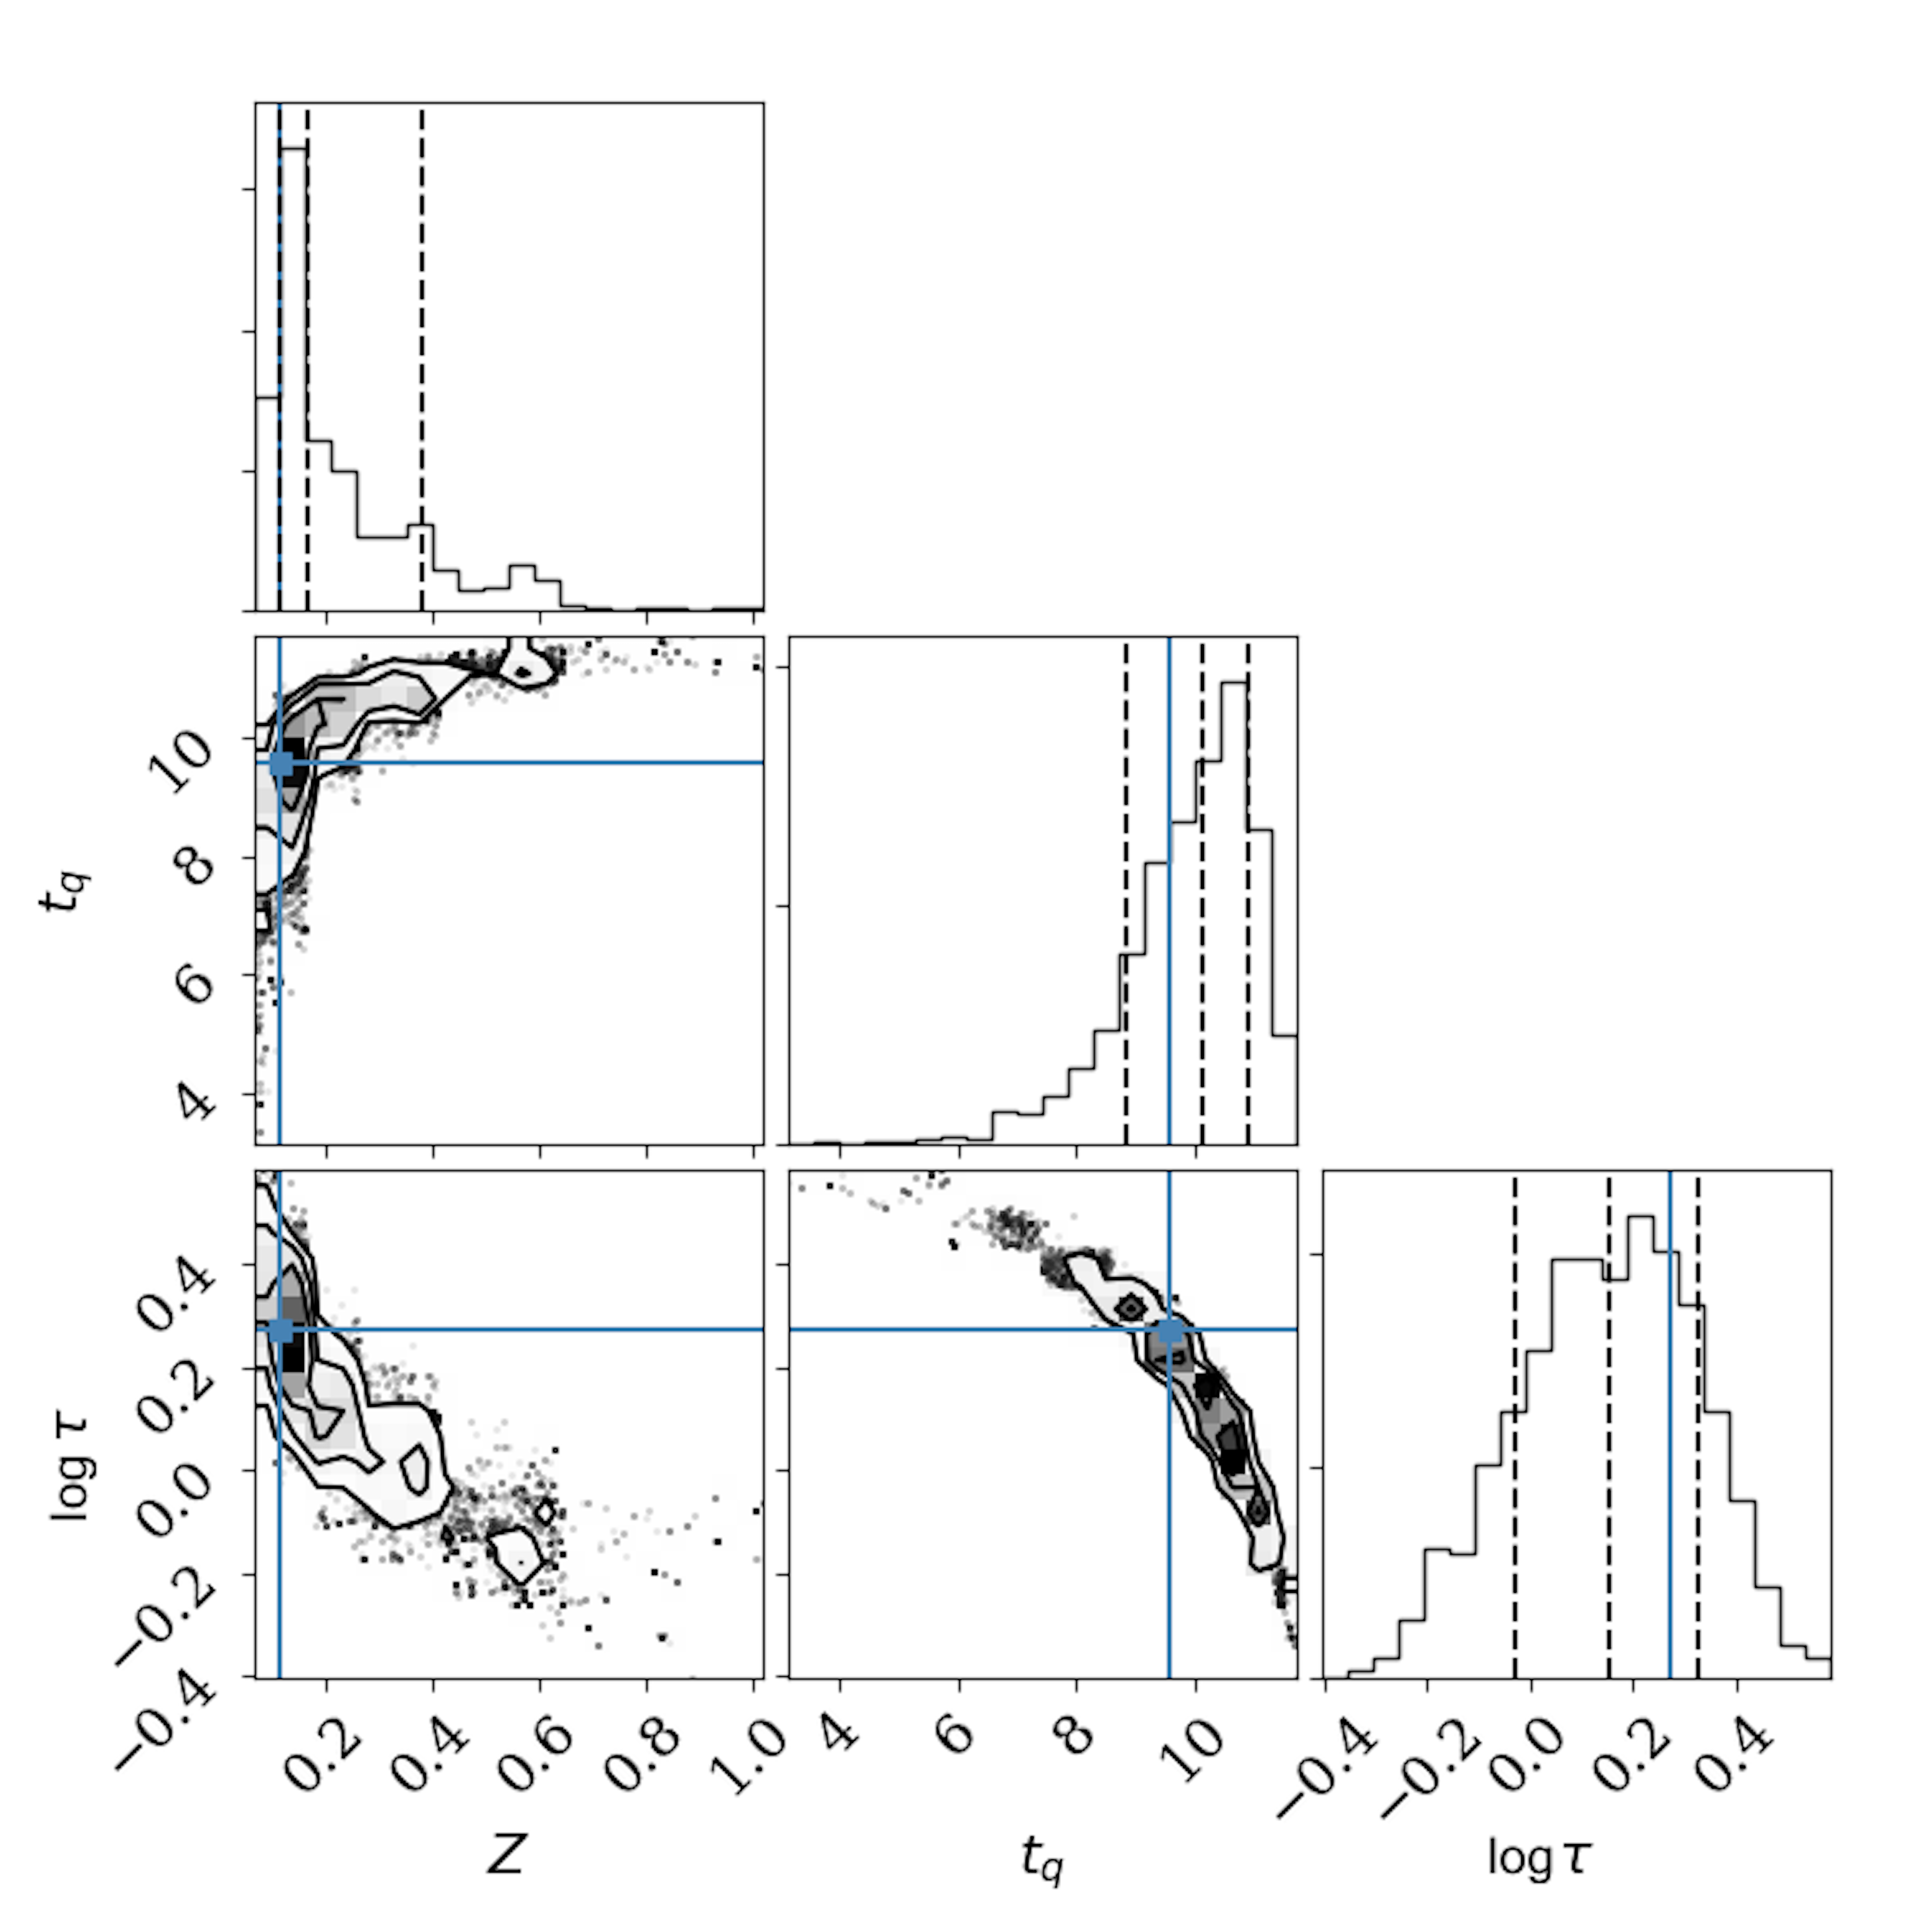
\includegraphics[width=\textwidth]{../figures/starpy_output_corner_example_20_newtqs_random_values.png}
\caption{Example output from \textsc{snitch} showing the posterior probability function traced by the MCMC walkers across the three dimensional parameter space $[Z, t_q, \log\tau]$. Dashed lines show the 18th, 50th and 64th percentile of each distribution function which can be interpreted as the `best fit' with $±1\sigma$. The blue lines show the known true values which \textsc{snitch} has managed to recover.}
\label{fig:output}
\end{figure*}

The walkers are all then ranked in order of decreasing average log likelihood, $\overline{l}_{(k)}$, or increasing $- \log \overline{l}_{(k)}$. If there are big jumps in the $- \log \overline{l}_{(k)}$, these are easy to spot and are indicative of areas where walkers have got stuck in local minima.The difference in $- \log \overline{l}_{(k)}$ for every adjacent pair of walkers is then calculated. The first pair whose difference is a certain amount times bigger than the average difference previously is then identified like so:
\begin{equation}
-\log \overline{l}_{(j+1)} + \log \overline{l}_{(j)} > Const − \frac{\log \overline{l}_{(j)} + log \overline{l}_{(1)}}{j - 1}.
\end{equation}



All the walkers with with $k>j$ are thrown away and only the ones with $k \leq j$ are kept after being identified as part of the global minimum. This can be seen in Figure~\ref{fig:comparepruning} wherein the walker positions at each step before pruning in the burn-in phase are shown in comparison to those after pruning in the main run stage. In the cases where the `walkers' did not get stuck in local minima, this pruning routine leaves the walker chains untouched. 

\begin{figure*}
\centering
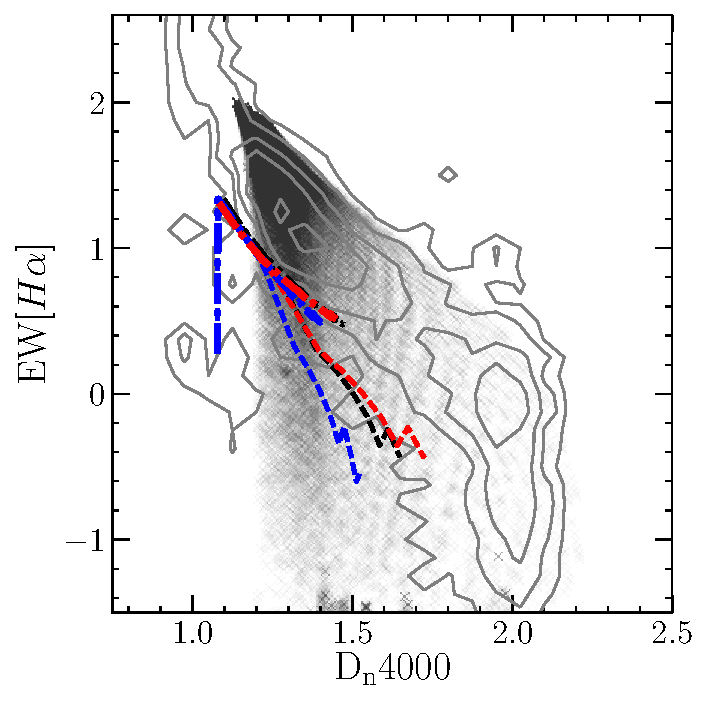
\includegraphics[width=0.24\textwidth]{../figures/marvin_dn4000_halpha_compare_sfhs.pdf}
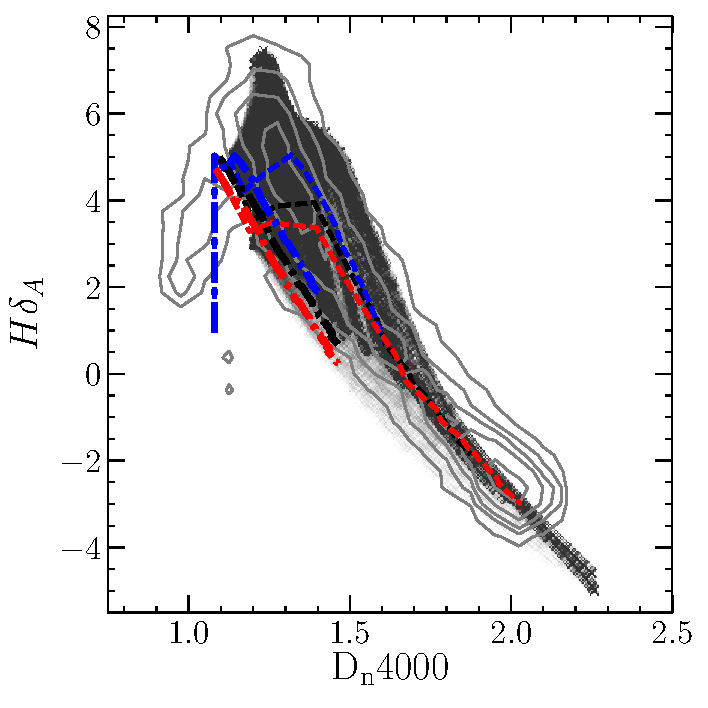
\includegraphics[width=0.24\textwidth]{../figures/marvin_dn4000_hdeltaa_compare_sfhs}
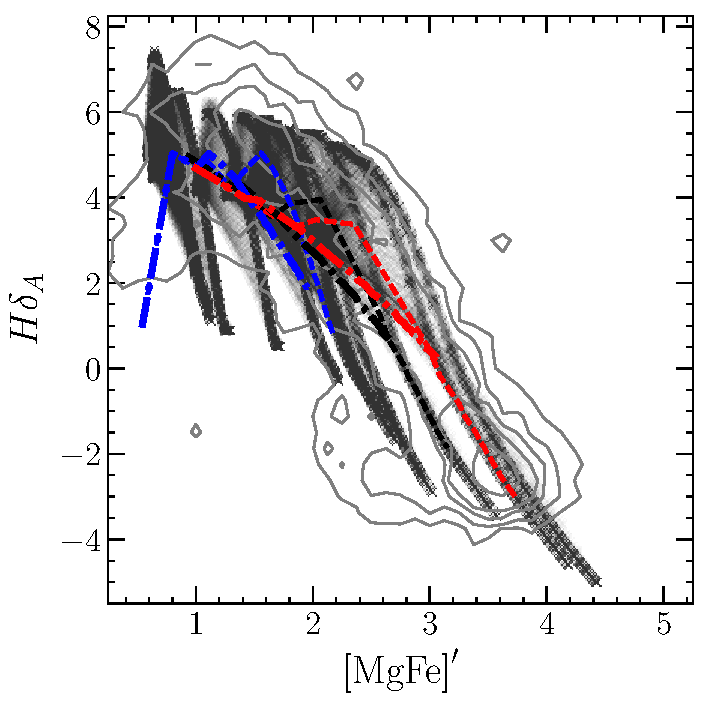
\includegraphics[width=0.24\textwidth]{../figures/marvin_mgfe_hdeltaa_compare_sfhs.pdf}
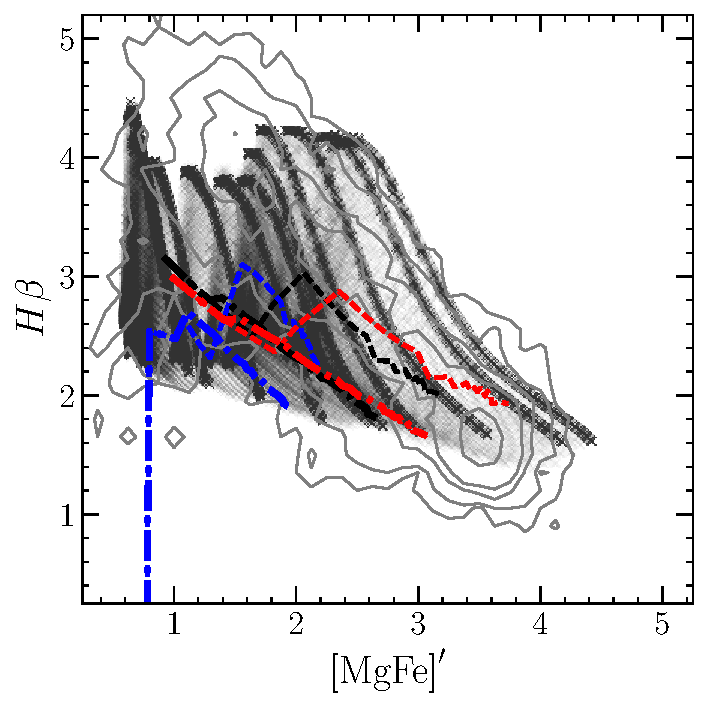
\includegraphics[width=0.24\textwidth]{../figures/marvin_mgfe_hbeta_compare_sfhs.pdf}
\caption{Validity test between actual spectral parameter measurements of the central spaxels (with $R/R_e < 0.1$) of all MPL-6 MaNGA galaxies (black contours) and those measured from the synthetic spectra generated for the look up table (red points; see Section~\ref{sec:emcee}). The contours enclose $(11, 39, 68, 86, 96)\%$ of the spaxel measurements in each panel. We have not attempted to recreate the distributions across spectral parameter space seen for real galaxies, we are merely showing the spectral parameters for the SFHs we happen to have generated across the 4-dimensional look up table, which we have shown in Figure~\ref{fig:rainbow} are degenerate.}
\label{fig:compare_manga_specmeas}
\end{figure*}

\section{Output of Code}\label{sec:output}


% \begin{table*}
% \centering
% \caption{The mean uncertainties ($\pm1±\sigma$) on the best fit and difference in known and best fit values ($\Delta [Z, t_q, \tau]$) for the 10 synthesised galaxy spectra returned when each spectral feature is omitted in turn.}
% \label{table:missingtestone}
% \begin{tabular*}{0.9\textwidth}{r@{\extracolsep{\fill}}|ccccccc}
% Spectral feature omitted ~          & None & $\rm{H}\alpha$ & $D_n4000$ & $\rm{H}\beta$ & $\rm{H}\delta_A$ & MgFe' \\ \hline
% Average uncertainty, Z $1\sigma$~ &   $0.1$  &   $0.1$                    &  $0.1$       &   $0.1$             &   $0.1$               & $0.2$ \\
% Average uncertainty, $t_q$ $1\sigma~$ &  $0.2$   &  $0.6$                       &   $0.5$      &    $0.2$            &   $0.3$               & $0.1$ \\
% Average uncertainty, $\tau$ $1\sigma~$ &   $0.1$   &  $0.4$                       &     $0.2	$    &   $0.1$             &   $0.1$               & $0.1$ \\ \hline
% $\Delta Z~\rm{[Gyr]}~$  &  $0.1$  & $0.1$ & $0.1$ & $0.1$ & $0.2$ & $0.2$ \\
% $\Delta t_q~\rm{[Gyr]}~$ &  $0.3$  & $1.3$ & $1.6$ & $0.8$ & $2.3$ & $2.5$ \\
% $\Delta \tau~\rm{[Gyr]}~$ & $0.2$ & $0.3$ & $0.5$ & $0.4$ & $0.9$ & $0.7$
% \end{tabular*}
% \end{table*}

\begin{table*}
\centering
\caption{The mean uncertainties ($\pm1±\sigma$) on the best fit and difference in known and best fit values ($\Delta [Z, t_q, \tau]$) for the 10 synthesised galaxy spectra returned when each spectral feature is omitted in turn.}
\label{table:missingtestone}
\begin{tabular*}{0.9\textwidth}{r@{\extracolsep{\fill}}|ccccccc}
Spectral feature omitted ~          & None & $\rm{H}\alpha$ & $D_n4000$ & $\rm{H}\beta$ & $\rm{H}\delta_A$ & MgFe' \\ \hline
Average uncertainty, Z $1\sigma$~ &  $0.2$ &  $0.3$ &  $0.2$ & $0.2$ & $0.2$ & $0.4$ \\
Average uncertainty, $t_q$ $1\sigma~$ & $1.1$ & $1.9$ & $1.7$ & $2.1$ & $3.2$ & $2.4$ \\
Average uncertainty, $\tau$ $1\sigma~$ & $0.4$ & $0.8$ & $0.9$ & $0.5$ & $0.5$ & $0.8$ \\ \hline
$\Delta Z~\rm{[Gyr]}~$  &  $0.1$  & $0.1$ & $0.3$ & $0.2$ & $0.1$ & $0.3$ \\
$\Delta t_q~\rm{[Gyr]}~$ &  $0.3$  & $1.3$ & $1.6$ & $1.5$ & $1.9$ & $0.8$ \\
$\Delta \tau~\rm{[Gyr]}~$ & $0.2$ & $2.3$ & $1.4$ & $2.1$ & $2.6$ & $1.5$
\end{tabular*}
\end{table*}


The burn-in and main run walker positions and posterior probabilities at each step are written to disc by \textsc{snitch}. From this three dimensional MCMC chain charting the $[Z, t_q, \log \tau]$ positions of the walkers around parameter space, the `best fit' $[Z, t_q, \log \tau]$ values along with their uncertainties can be determined from the 16th, 50th and 84th percentile values of the walker positions. An example output from \textsc{snitch} for a single synthetic spectrum constructed with the FSPS models (see Section~\ref{sec:fsps}) is shown in Figure~\ref{fig:output}. This figure is also written to disc by \textsc{snitch} upon completion of a run on a single spectrum.  


The routine outlined in Section~\ref{sec:code} has been released as an open source package named \textsc{snitch}\footnote{\url{http://www.github.com/rjsmethurst/snitch/}}. The required inputs for \textsc{snitch} to run on a single spectrum are at least one, if not all, of $\rm{EW}[H\alpha]$, $\rm{D}_n4000$, $\rm{H}\beta$, $\rm{H}\delta_A$ and MgFe' and their associated errors and the spectrum redshift, $z$. 

\section{Testing}\label{sec:test}

\subsection{Validation of spectral parameter measurements}\label{sec:precisiontest}


Before testing the performance of the code, we tested the validity of the measurements of the spectral parameters generated in the look up table (see Section~\ref{sec:emcee} and Figure~\ref{fig:rainbow}) for the synthetic spectra generated by FSPS. To do this, we collated the spectral parameters for all the central spaxels (with $R/R_e < 0.1$ to give a reasonable sample size) of all MPL-6 MaNGA galaxies. These are shown by the black contours in each of the panels of Figure~\ref{fig:compare_manga_specmeas}. These are overlaid over points showing the spectral measurements for the synthetic FSPS spectra from the generated look up table. We can see that similar ranges are found for the modelled SFHs as for the spaxels of real MaNGA galaxies, suggesting that the models produced are appropriately generated and measured. Note that whilst the black contours are representative of the distribution of real spectral parameters in MaNGA galaxies, the red points of the model SFHs are just those generated in the look up table. Therefore, we have not attempted to recreate these real distributions across spectral parameter space, merely we are showing the spectral parameters for the SFHs we happen to have generated across the 4-dimensional look up table. 




\subsection{Testing precision}\label{sec:precisiontest}

% \begin{figure*}
% \centering
% \includegraphics[width=\textwidth]{../code/test_precision_mosaic/mosaic_spec_starpy_testing_one_log_powell.pdf}
% \caption{Results from \textsc{snitch} for an array of synthesised galaxies with known true $[Z, t_q, \log \tau]$ values (marked by the solid red lines) assuming an error on the input spectral measurements of the average error on the measured MaNGA spectra measurements. $Z$ values were set to solar with some gaussian noise, whereas $t_q$ and $\tau$ values have been set across a regular grid to observe how \textsc{snitch} performs across the various areas of parameter space. Pruning has been applied to the plotted walker positions, from which `best fit' parameters have been derived, shown by the solid blue lines. In each case \textsc{snitch} has succeeded in locating the true parameter values within the degeneracies of the SFH model.}
% \label{fig:test_mosaic}
% \end{figure*}


In order to test that \textsc{snitch} can find the correct quenched SFH model for a given set of spectral features, 25 synthesised galaxy spectra were created with known SFHs (i.e. known randomised values of $\theta = [Z, t_q, \log \tau]$) from which spectral features were generated using the FSPS models (see Section~\ref{sec:fsps}). These were input into \textsc{snitch} to test whether the known values of $\theta$ were reproduced, within error, for each of the 25 synthesised galaxies. %Figure~\ref{fig:test_mosaic} shows the results for each of these synthesised galaxies, with the known values of $\theta$ shown by the red lines. Figure~\ref{fig:test_mosaic} shows how the spread in the walker positions gets broader as the inferred $\tau$ value gets larger (i.e. longer quench) and the inferred $t_q$ value gets smaller (i.e. earlier quench). 
In all cases the true values reside within the parameter space explored by the walkers left over after pruning, which trace the global minimum of the posterior probability. \textsc{snitch} therefore succeeds in locating the true parameter values within the degeneracies of the SFH model for known values. However, the spread in the walker positions gets broader as the inferred $\tau$ value gets larger (i.e. longer quench) and the inferred $t_q$ value gets smaller (i.e. earlier quench).  This test therefore demonstrates how \textsc{snitch} is precise in recovering known SFHs, however that precision varies across the parameter space. The median difference between known and inferred paramter values for 25 random SFHs is $[\Delta Z,~\Delta t_q,~\Delta \tau]~=~[0.1~\rm{Z}_{\odot},~0.3~\rm{Gyr},~0.2~\rm{Gyr}]$ and the maximum difference between the inferred and true values are $[\Delta Z,~\Delta t_q,~\Delta \tau]~=~[0.7~\rm{Z}_{\odot},~3.7~\rm{Gyr},~1.4~\rm{Gyr}]$.


\subsection{Testing precision when less spectral information provided}\label{sec:missingtest}



\textsc{snitch} is designed so that not all of the spectral features have to be provided for the code to return an inferred quenching history. This is a particularly useful feature if the user is unable to obtain or measure a certain spectral feature, if for example, measurements are being obtained from archival data or a feature lies outside of the wavelength range of their spectrum. 

Users should note that quenching histories inferred given less inputs results in a larger uncertainty on the quoted best fit parameters returned by \textsc{snitch}. To quantify this we generated 10 random $[Z, t_q, \log \tau]$ values and used them to generate synthetic spectra the measurements for which we ran through \textsc{snitch}, each time omitting one of the spectral features from the list of inputs. The mean uncertainties on the best fit and difference between known and best fit values returned when each spectral feature is omitted are quoted in Table~\ref{table:missingtestone}. 

For further combinations of missing parameters, we suggest the user completes their own tests to determine how the quoted uncertainty will change with the omission of more than one spectral feature. However, we do not recommend using \textsc{snitch} if the number of available spectral features is less than $4$. If this is the case, the number of inputs given to the code will be equal to or less than the number of parameters to be inferred and the inferred SFH will be unreliable. 

\subsection{Population testing}\label{sec:poptest}

\begin{figure*}
\centering
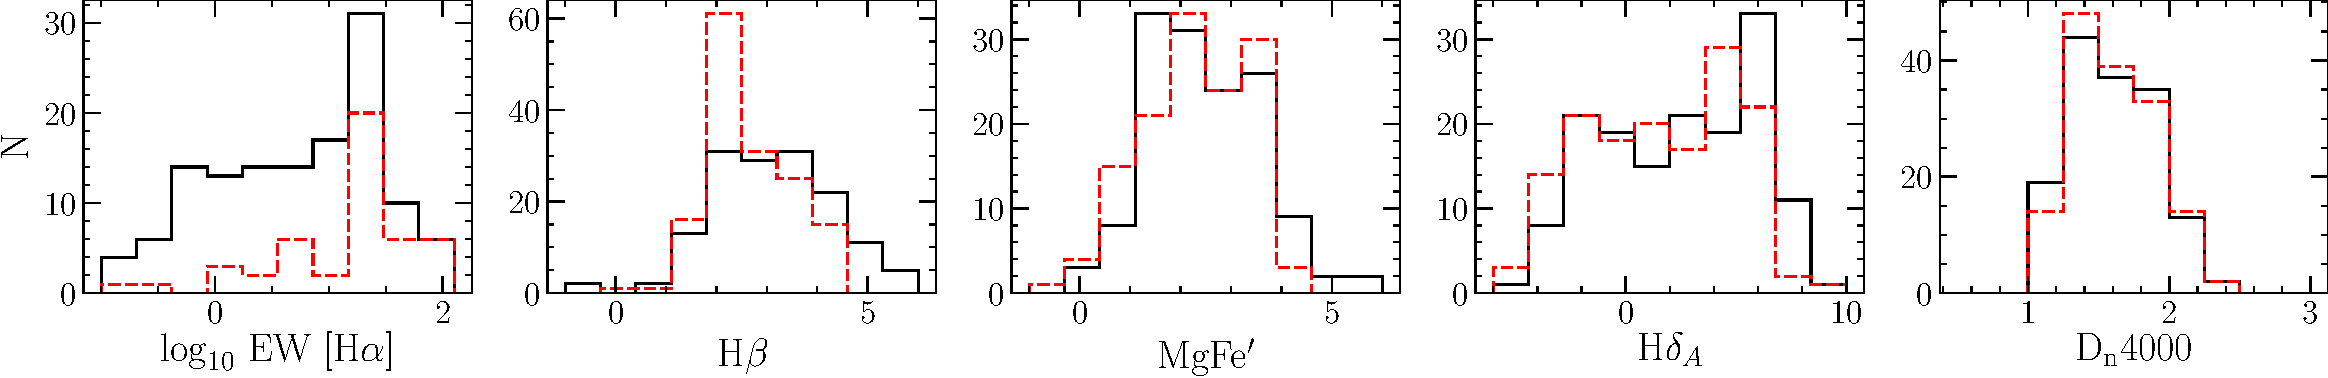
\includegraphics[width=\textwidth]{../figures/population_test_compare_results_gaussian_noise_sfr_limited.pdf}
\caption{The distribution, from right to left of the $\log_{10}$EW$[\rm{H}\alpha]$, $H\beta$, $\rm{MgFe'}$, $\rm{H}\delta_A$ and $\rm{D_n4000}$ values of a random spaxel in each of $150$ randomly selected observed MaNGA galaxies (black solid line). In each panel the distribution of the \textsc{snitch} inferred spectral parameter is shown by the red dashed line.}
\label{fig:mangacompare}
\end{figure*}


A further test of \textsc{snitch} is to determine whether the inferred SFH parameters of $[Z,~t_q,~\log\tau]$ can reproduce the distribution of spectral parameters of a number of galaxy spectra. We randomly selected a spaxel from each of $150$ MaNGA MPL-6 galaxies  and used the measured spectral parameters provided by the DAP as inputs to \textsc{snitch}. We then used the inferred SFHs returned by \textsc{snitch} to estimate inferred spectral parameters for each of the spaxels from the $150$ galaxies. We also added a random multiple, drawn from a Gaussian distribution with mean of $0$ and standard deviation of $1.1$ (i.e. normally distributed between roughly $-3$ and $3$ so that the noise added to the inferred value is $\pm3\sigma$), of the error on each measured spectral parameter to the inferred value.

Figure~\ref{fig:mangacompare} shows the distributions of the inferred and measured spectral parameters and highlights how the inferred values trace the original measured values well, at least for the absorption features. However, we can see that \textsc{snitch} struggles to reproduce the distribution of $\log_{10}$EW$[\rm{H}\alpha]$. This is due to the fact that the look up tables which \textsc{snitch} uses are masked for $\log_{10}$EW$[\rm{H}\alpha]~\lesssim~1$ (see left most panel of Figure~\ref{fig:rainbow}) as these values become unreliable measurements due to the contamination from the nearby $[NII]$ doublet. Therefore \text{snitch} will return \texttt{nan} for these SFHs where star formation is minimal. This was true for $92$ of the $150$ galaxy spaxels. We did not mask the measured EW$[\rm{H}\alpha]$ values for the observed parameters in order to provide \textsc{snitch} with 5 inputs for each MaNGA galaxy, as a control. See Section~\ref{sec:missingtest} wherein we describe how the performance of \textsc{snitch} was tested when each spectral parameter was omitted in turn from the list of inputs. 

\subsection{Testing accuracy}\label{sec:accuracytest}

We have shown in the previous section that \textsc{snitch} can return precise known values for SFHs, however now we must test its accuracy. In order to quantify this we have run \textsc{snitch} on spectra which have previously derived star formation histories. Firstly, on those which have had toy models derived (Section~\ref{secsec:compare}) and then on spectra with star formation histories from hydrodynamic simulations (Section~\ref{sec:lgalaxies}).

\subsubsection{Comparing with other toy model SFH codes}\label{secsec:compare}

\begin{figure}
\centering
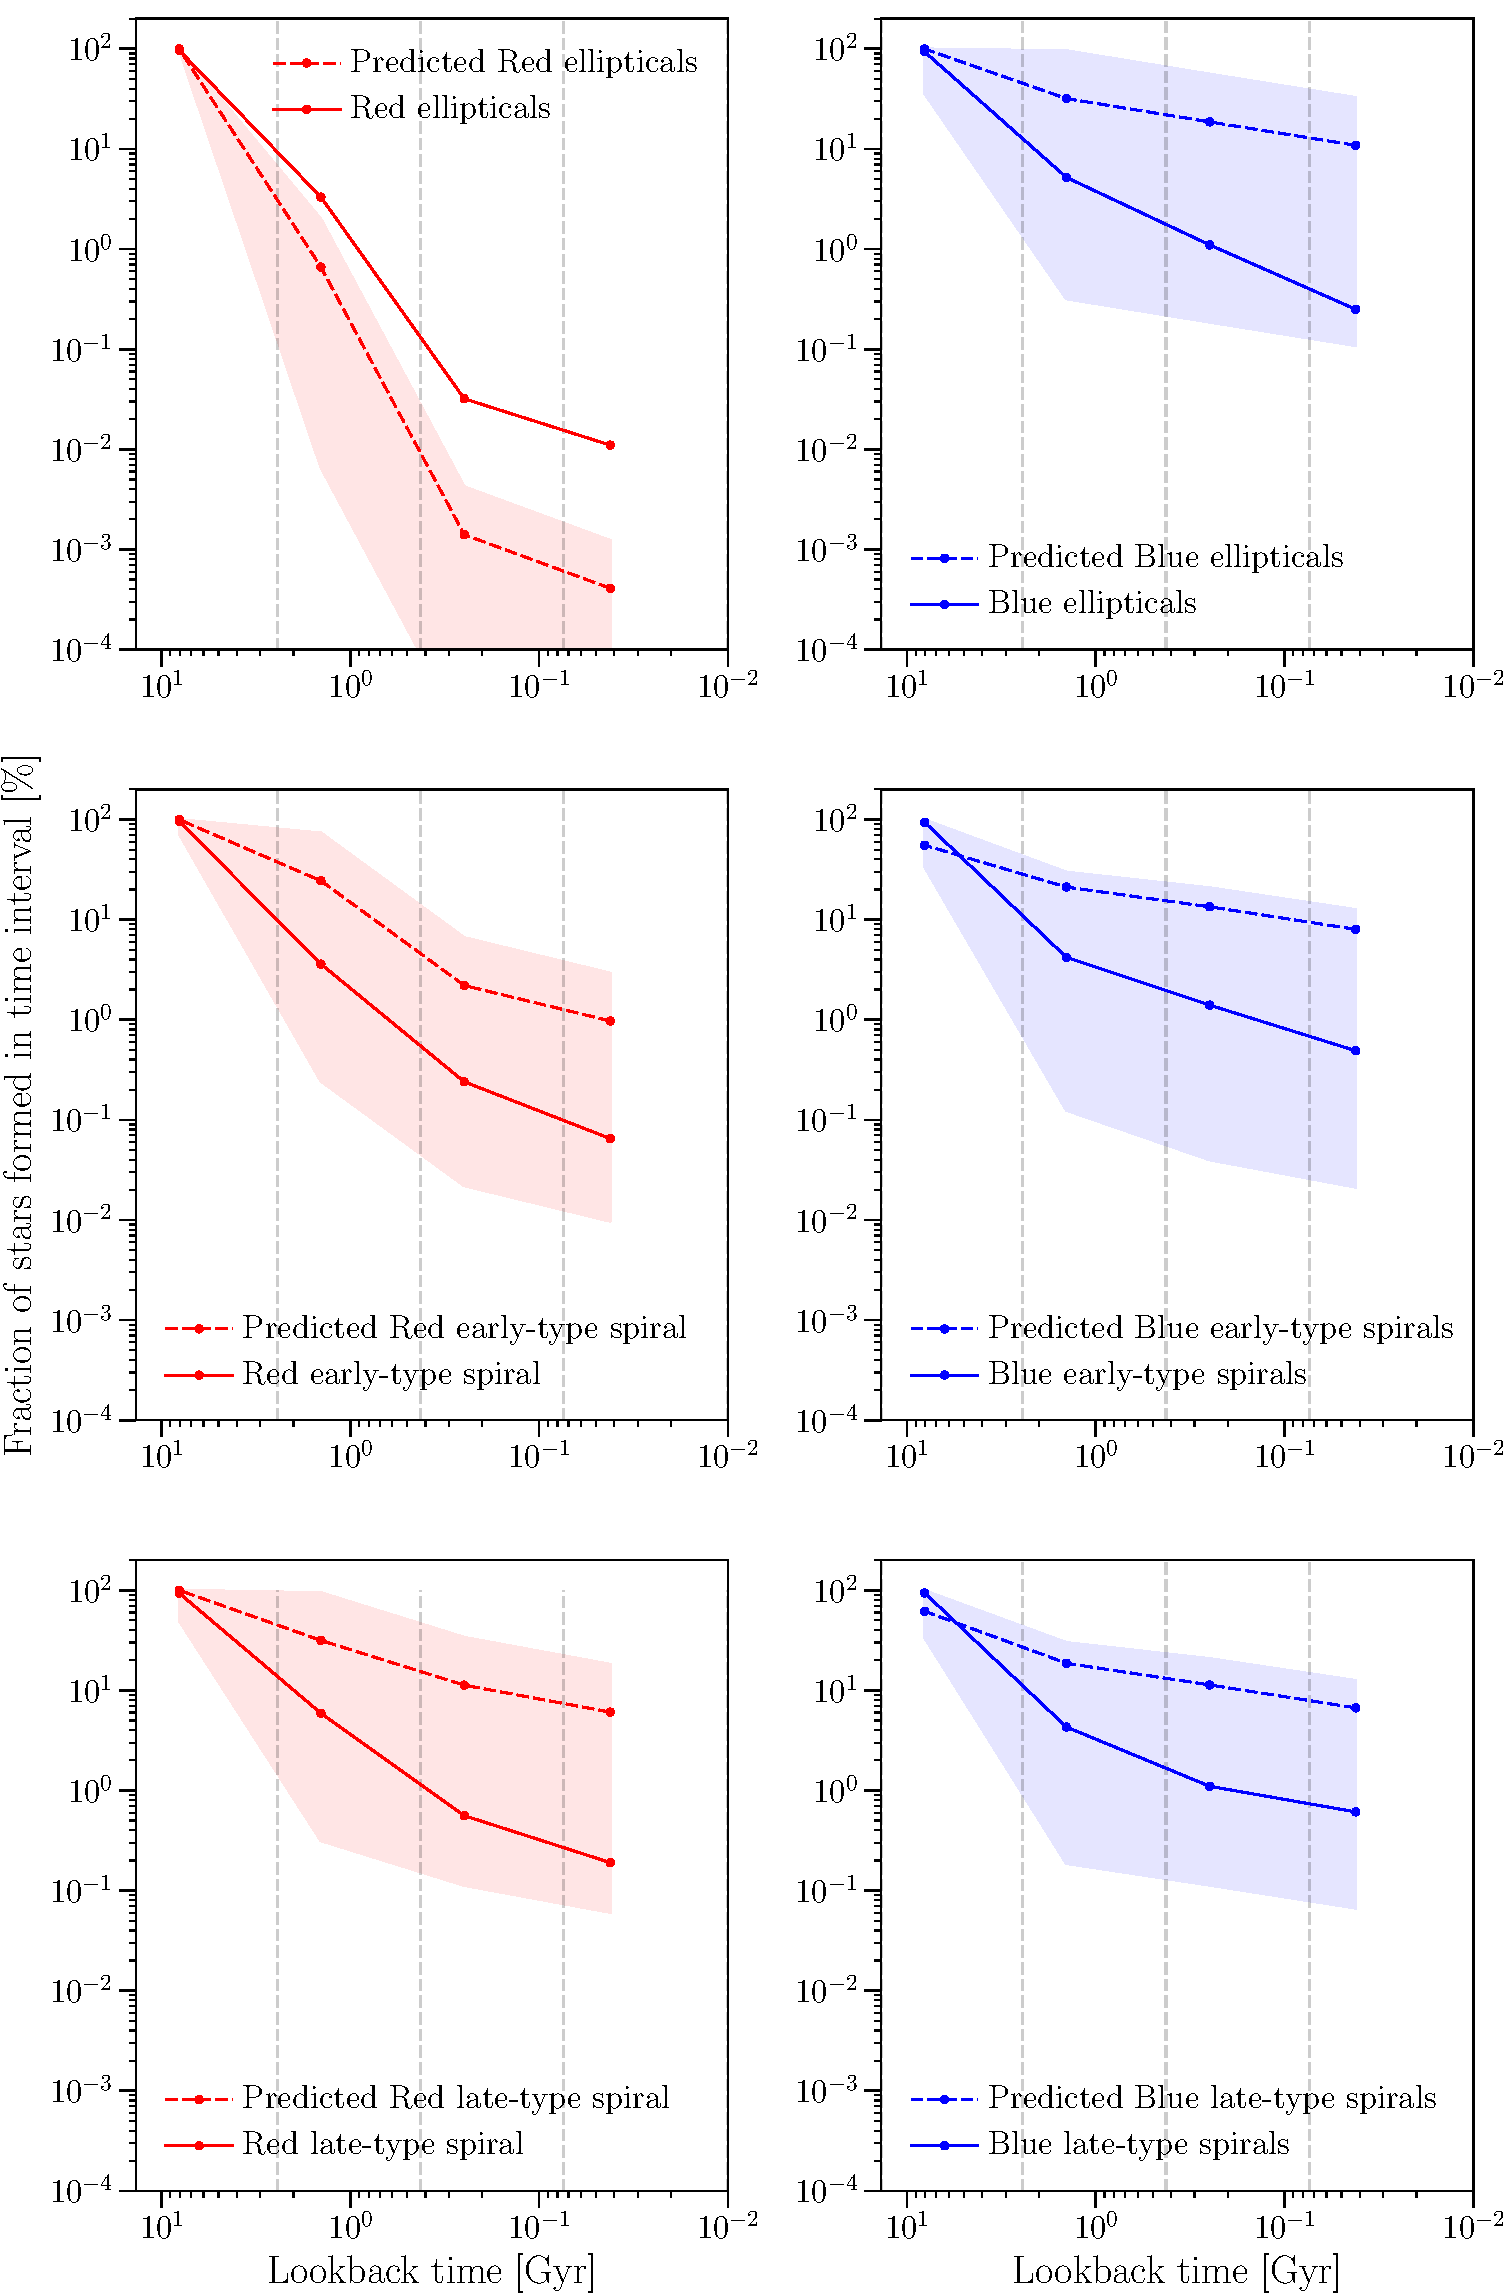
\includegraphics[width=0.48\textwidth]{../code/test_tojiero/compare_tojeiro_pred_results.pdf}
\caption{The mean star formation fraction (SFF) in each age bin for the six galaxy samples analysed by \protect\cite[][solid lines]{tojeiro13} and returned by \textsc{snitch} (dashed lines). The shaded region shows the $1\sigma$ error on the predicted SFF inferred by \textsc{snitch}.}
\label{fig:tojeirocompare}
\end{figure}

In the case of the previously fitted toy models, we have compared the results of \textsc{snitch} with the toy star formation histories derived by \cite{tojeiro13} for $6$ stacked SDSS spectra of $13959$ red ellipticals, $381$ blue ellipticals, $5139$ blue late-type spirals, $294$ red late-type spirals, $1144$ blue early-type spirals and $1265$ red early-type spirals. We measured the spectral features of each of the $6$ stacked spectra using the method outlined in Section~\ref{sec:dap} and input them into \textsc{snitch}. Since \cite{tojeiro13} quoted their results in terms of the fraction of stars formed (SFF) in a given time period, we have followed the same method. In Table~\ref{table:tojeirocompare} we have listed the SFF for the six samples used by \citeauthor{tojeiro13} and the SFF for the best fit parameters returned by \textsc{snitch} along with the median $1\sigma$ error. These results are also plotted in Figure~\ref{fig:tojeirocompare}. 

We can see from these results that \textsc{snitch} broadly agrees with the results of \cite{tojeiro13}, within error for the red galaxy stacked spectra, i.e. those galaxies which typically have lower star formation rates. However, \textsc{snitch} does not agree with the star formation fractions derived by \cite{tojeiro13} for blue galaxies. This is to be expected since \textsc{SNITCH} fits a quenching SFH model to a galaxy spectrum and so would return a less accurate SFH for star forming spectra (see Section~\ref{secsec:starforming}). These results suggest that \textsc{SNITCH} does return an accurate toy model of star formation history at least for galaxies which are quenching or quenched.   



\begin{table*}
\centering
\caption{The mean star formation fraction (SFF) in each age bin for the six galaxy samples quoted by \protect\cite[][TSFF]{tojeiro13} and returned by \textsc{snitch}. Each value is quoted with a $1\sigma$ uncertainty, for the \protect\cite{tojeiro13} values this is quoted as the standard error on the mean for each bin . The SFF and $1\sigma$ errors are given in units of $10^{-3}$.}
\label{table:tojeirocompare}
\begin{tabular*}{0.9\textwidth}{l|cc|cc|cc|cc}
                        & \multicolumn{2}{c|}{$0.01 - 0.074~\rm{Gyr}$}     & \multicolumn{2}{c|}{$0.074 - 0.425~\rm{Gyr}$} & \multicolumn{2}{c|}{$0.425 - 2.44~\rm{Gyr}$} & \multicolumn{2}{c}{$2.44 - 13.7~\rm{Gyr}$} \\ \hline
                        & TSFF & \multicolumn{1}{c|}{\textsc{snitch} SFF} & TSFF          & \textsc{snitch} SFF          & TSFF          & \textsc{snitch} SFF         & TSFF         & \textsc{snitch} SFF        \\ \hline
Red ellipticals         & 0.11   &  1 $\pm$ 50  &  0.32  &    1 $\pm$ 51   &  12   &   24 $\pm$ 62   &  966  &   973 $\pm$ 42    \\
Red early-type spirals  & 0.65   &  5 $\pm$ 53  &  2.4   &  13 $\pm$ 57     &  36   &   238 $\pm$ 169   &  960  &  741 $\pm$ 75    \\
Red late-type spirals   &  1.9   &  75 $\pm$ 87   &  5.6   &   136 $\pm$ 118    &  59   &   323 $\pm$ 212   &  933  &   445 $\pm$ 222    \\ \hline
Blue ellipticals        &  2.5   &  109 $\pm$ 105   &  11    &   188 $\pm$ 144    &  52   &   333 $\pm$ 211   &  934  &     350 $\pm$ 271  \\
Blue early-type spirals &  4.9   &  84 $\pm$ 58  &  14    &   140 $\pm$ 96    &  42   &   217 $\pm$ 134   &  938  &  537 $\pm$ 301     \\
Blue late-type spirals  &  6.1   &  72 $\pm$ 61  &  11    &   123 $\pm$ 102    &  43   &    201 $\pm$ 148  &  939  & 585 $\pm$ 322                              
\end{tabular*}
\end{table*}

% \subsubsection{Comparing with full spectral fitting codes}\label{secsec:fullcompare}


% For the case of the full spectral fit derived star formation history, we have chosen three examples from work by \cite{?} in the MaNGA team. The sample used by \citeauthor{?} have had their spectra fit and measured using the full MaNGA DAP pipeline \citep{westfall18} so measurements of their spectral features were readily available. We used these measurements as inputs into \textsc{snitch} and in Figure~\ref{fig:fspfcompare} have plotted the output best fit quenching history in comparison to that output by the full spectra fitting code of \cite{?}. This figure shows that although we implement a toy model of star formation history in \textsc{snitch}, we are able to recover the features of the most recent epoch of star formation.  

\subsubsection{Comparing with `realistic' known SFHs from hydrodynamic simulations}\label{sec:lgalaxies}

\begin{figure}
\centering
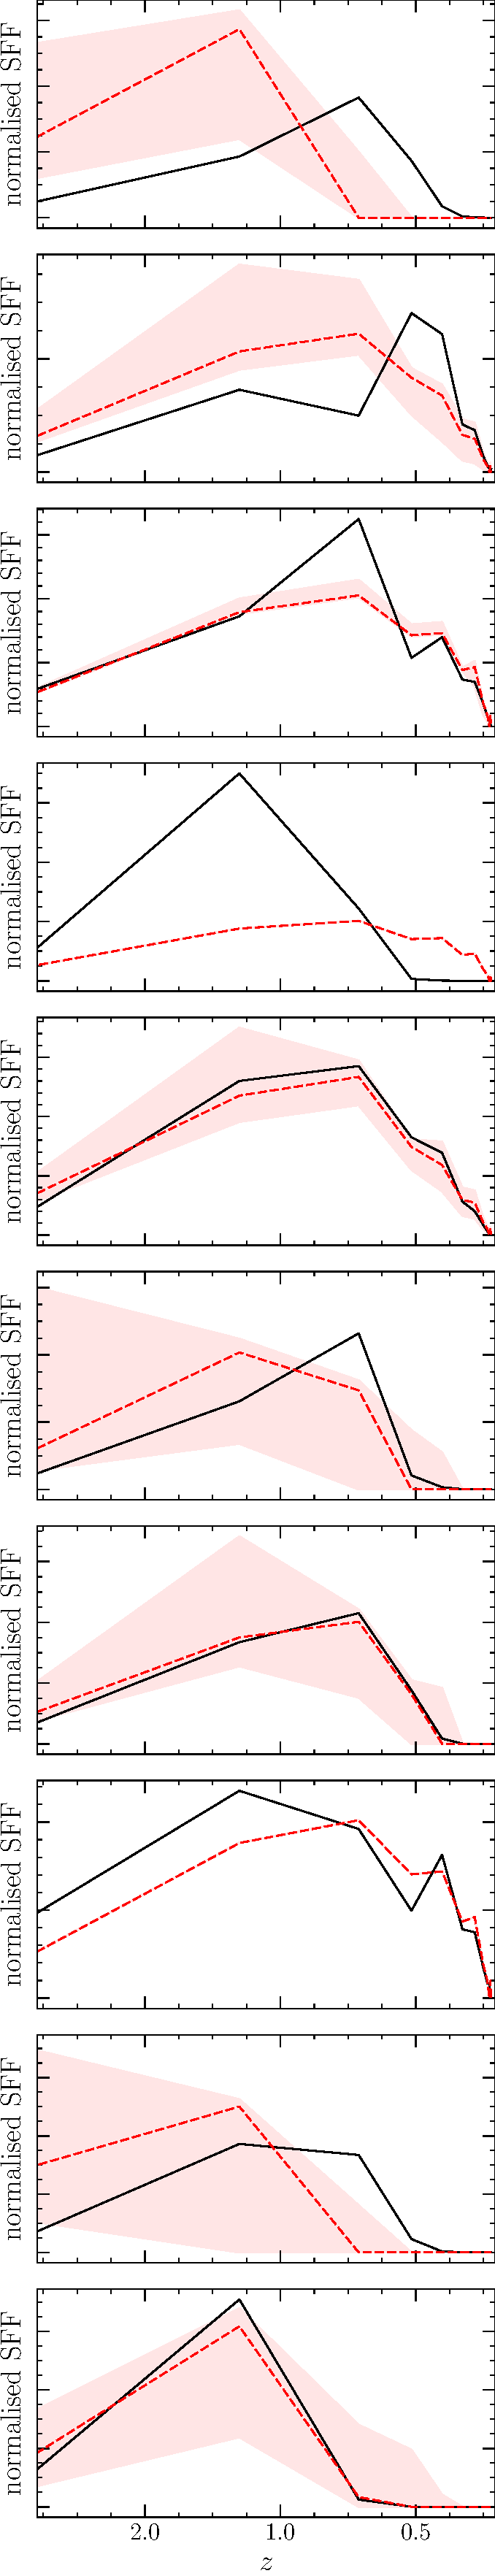
\includegraphics[height=0.91\textheight]{../figures/compare_black_Lgal_quasar_sff_inferred_sfh_red.pdf}
\caption{Comparison of the SFFs generated by \texttt{Lgalaxies} (black) and those inferred by \textsc{snitch} (red, dashed with shaded uncertainty regions) for $10$ randomly selected synthetic spectra with SFRs in the range $0~<~\rm{SFR}~[M_{\odot}~\rm{yr}^{-1}]~<~1$, and stellar masses $10^9~<~M_{*}~[M_{\odot}]~<~10^{11}$. Note how \textsc{snitch} is sensitive to the most recent change in the SFF.}
\label{fig:lgalsfhs}
\end{figure}

\begin{figure}
\centering
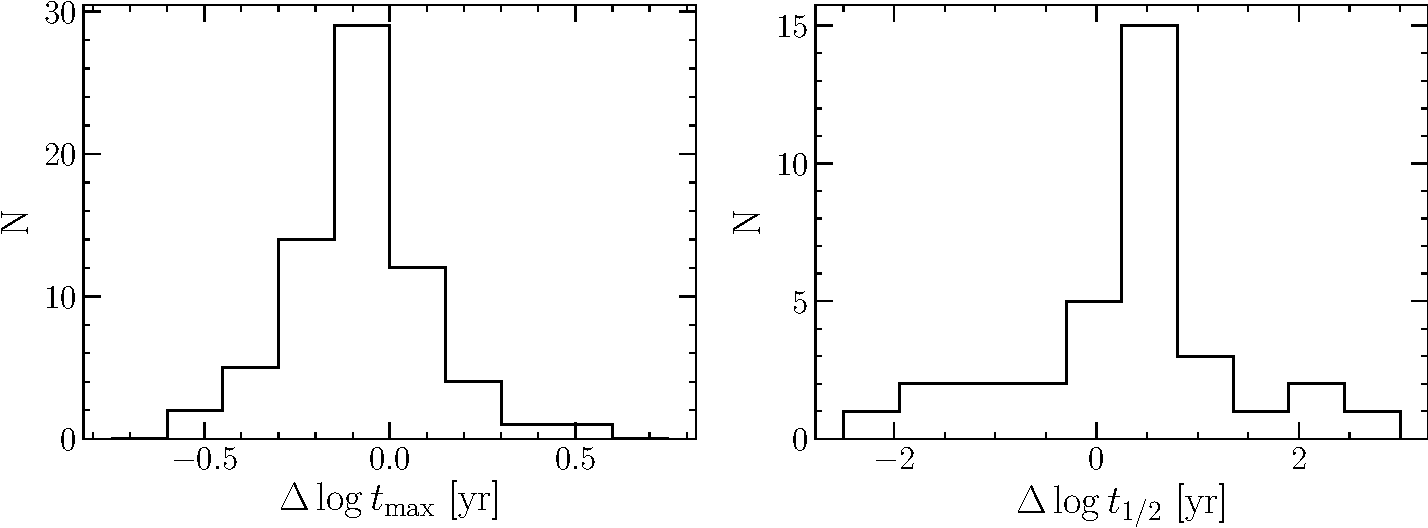
\includegraphics[width=0.49\textwidth]{../figures/compare_difference_in_t_at_max_SFR_and_t_for_SFR_to_drop_to_half_max.pdf}
\caption{Comparison of the difference between the calculated and inferred time of maximum SFR ($\Delta \log t_{\rm{max}}$; left) and time for the SFR to drop to half of the maximum value ($\Delta \log t_{1/2}$; right) for the $104$ synthetic SFHs with a non zero quasar accretion rate generated by \texttt{LGalaxies}.}
\label{fig:genlgalsfhs}
\end{figure}

We generated $8238$ simulated galaxy SFHs using the \texttt{LGalaxies} suite of hydrodynamic simulations \citep{henriques15} at a redshift of $z=0.043$ (the mean redshfit of the MaNGA DR14 sample) with a range of star formation rates, $0 < \rm{SFR}~[M_{\odot}~\rm{yr}^{-1}] < 1$, and stellar masses $10^9 < M_{*} [M_{\odot}] < 10^{11}$. Of these $8238$ simulated galaxies we selected all of those flagged by \texttt{LGalaxies} to have a quasar accretion rate above zero. This resulted in $104$ simulated galaxies SFHs. We used the FSPS models of \cite{conroy10} to generate synthetic spectra for each of these $104$ simulated SFH (as described in Section~\ref{sec:fsps}) and then measured their spectral features using the MaNGA DAP functions outlined in Section~\ref{sec:dap}. We then input these measurements into \textsc{snitch} to derive the best fit $[Z, t_q, \log \tau]$ parameters for our toy model of SFH to compare with the known SFH output by the hydrodynamic simulation. This test is therefore very similar to our tests with different known SFHs that we generated in Section~\ref{sec:diffSFHs}, however the SFHs generated by the hydrodynamic simulation can be classed as both more varied and more ``realistic" in this case.

Figure~\ref{fig:lgalsfhs} shows the normalised star formation fractions as generated by \texttt{Lgalaxies} and inferred for their spectra by \textsc{snitch} for $10$ randomly selected simulated SFHs. We can see that the output from \textsc{snitch} largely agrees, within the uncertainties, with the known SFHs of Lgalaxies. Although not all details of the \texttt{Lgalaxies} SFHs are reproduced, \textsc{snitch} identifies the most recent epoch of a dramatic change in the star formation rate.

We can also generalise the SFHs generated by \texttt{Lgalaxies} and returned by \textsc{snitch} into two parameters, the time of maximum SFR, $\log t_{\rm{max}}$, and the time for the SFR to drop to half of the maximum value ($\log t_{1/2}$). Note, that if a galaxy is still star forming then we cannot derive a value for $t_{1/2}$. These generalised parameters roughly trace the exponential SFH parameters of $t_q$ and $\tau$, but allow for a comparison to the SFHs generated by \texttt{Lgalaxies} which are not constrained to a specific form. Figure~\ref{fig:genlgalsfhs} shows the difference between the generated and inferred values of $\log t_{\rm{max}}$ \& $\log t_{1/2}$. We can see that for the majority of synthetic spectra the inferred generalised SFH parameters are comparable to those generated by \texttt{Lgalaxies}. However there is a much larger spread in $\Delta \log t_{1/2}$ (shown in the right panel of Figure ~\ref{fig:genlgalsfhs}) than in $\Delta \log t_{\rm{max}}$ (shown in the left panel), suggesting that for galaxies with more realistic SFHs, \textsc{snitch} will return a more accurate value for the time of quenching, $t_q$, than for the rate that quenching occurs, $\log \tau$.



\subsection{Testing performance with different SFH definitions}\label{sec:diffSFHs}

\subsubsection{Star Forming SFHs}\label{secsec:starforming}

We must also understand how \textsc{snitch} behaves when spectral parameters derived from a star forming spectra are input. For example, Figure~\ref{fig:sfgal} shows the example output from \textsc{snitch} across the three dimensional parameter space $[Z,t_q,\log \tau]$ for a synthetic galaxy spectrum which is still star forming at a constant rate by the time of observation. Note that the walkers have explored only the parameter space where $t_q > t_{obs}$, i.e. the observed redshift of the galaxy (see Section~\ref{sec:fsps}), and all possible values of $\log \tau$ since the synthetetic galaxy has not yet quenched and therefore all quenching rates are equally likely.  

\begin{figure}
\centering
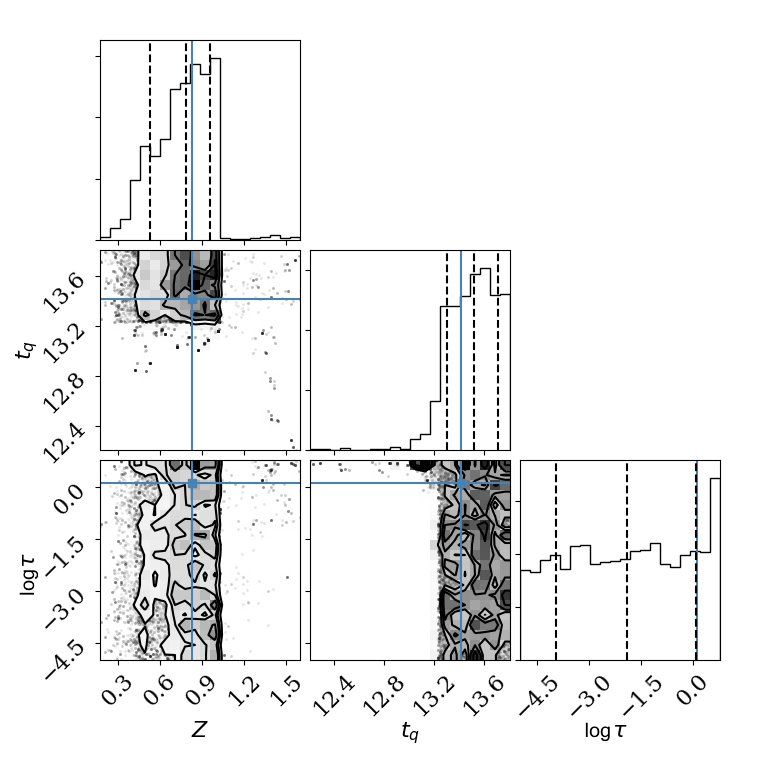
\includegraphics[width=0.475\textwidth]{../figures/starpy_output_corner_testing_SF_SFH_newtqs_random_values.png}
\caption{Example output from \textsc{snitch} showing the posterior probability function traced by the MCMC walkers across the three dimensional parameter space $[Z,t_q,\log \tau]$, for a synthetic galaxy spectrum which has a SFH with constant SFR.  Dashed lines show the 18th, 50th and 64th percentile of each distribution function which can be interpreted as the `best fit' with $1\sigma$. The blue lines show the known true values which snitch has managed to recover, within error. }
\label{fig:sfgal}
\end{figure}


\subsubsection{Different Forms of Quenching SFHs}

Obviously, not all galaxies will be accurately described by an exponentially quenching SFH. In special use cases (for example studying post starburst galaxies) a different SFH may be defined by the user by replacing the \texttt{expsfh} function with their own. 

However, we have also tested how \textsc{snitch} behaves when spectra with known SFHs of different forms are input. We tested spectra with  constant, burst, many burst, normal and log-normal models of SFH, all of which are often used in the literature to model simple SFHs. 

We found that \textsc{snitch} was always sensitive to the most recent epoch of star formation or quenching. For the constant SFR model, \textsc{snitch} returned a very recent $t_q$ and a very large $\tau$, i.e. a galaxy which has had constant SFR up until very recently at which point it started to decline very slowly. For the burst and many-burst models, \textsc{snitch} returns a constant SFR up until the peak of the last burst at which point quenching happens very rapidly. Similarly for the log normal and normal SFHs, \textsc{snitch} returns a best fit SFH with constant SFR until the peak of the normal and which point it declines at a rate comparable to the drop off of the Gaussian SFH. All of these tests suggest that \textsc{snitch} is most sensitive to the most recent epoch of star formation but can also roughly trace the quenching of star formation even if the true decline does not occur at an exponential rate. 

% \begin{figure}
% \centering
% \includegraphics[width=0.475\textwidth]{../figures/different_SFHs_to_test.png}
% \caption{The shapes of the different known SFHs input into \textsc{snitch}.}
% \label{fig:differentSFHs}
% \end{figure}


\section{Conclusions}

We have described our quenching history inference code \textsc{snitch} (bayeSian iNference, given emIssion and absorpTion spectral features, of quenChing Histories) which uses absorption and emission features measured from a spectra to infer a simple exponentially declining toy model of star formation history. We have demonstrated that it is both precise and accurate at deriving a toy model of star formation history. We have completed a rigorous set of tests the results of which suggest that \textsc{snitch} is most sensitive to the most recent epoch of star formation but can also trace the quenching of star formation even if the true decline does not occur at an exponential rate.  We advocate the use of this code as a comparative tool across a large sample of spectra, rather than to derive a detailed star formation history of a single spectra. 

\bibliographystyle{mn2e}
\bibliography{refs}  

\end{document}
